
%(BEGIN_QUESTION)
% Copyright 2011, Tony R. Kuphaldt, released under the Creative Commons Attribution License (v 1.0)
% This means you may do almost anything with this work of mine, so long as you give me proper credit

Shown here is a typical 2-wire RTD bridge circuit, where the RTD is located a considerable distance away from the bridge circuit:

$$\includegraphics[width=15.5cm]{i00413x01.eps}$$

The two-wire cable connecting the RTD to the rest of the bridge circuit has resistance distributed along its length, shown in the schematic in ``lumped'' form as two ``$R_{wire}$'' resistors.  What effect will the presence of this cable resistance have on the temperature measurement system?  Will it result in a zero shift, a span shift, or both?  Why??

Calculate the output voltage of this bridge circuit when the 100 $\Omega$ RTD is at its reference temperature of 0$^{o}$ C, and each $R_{wire}$ resistance is equal to 2 $\Omega$ (Hint: the alpha figure is irrelevant in this problem).  

Also calculate how hot the RTD ``appears'' to be as indicated by the output voltage of the bridge circuit, given the added cable resistance.  Assume a European $\alpha$ value for this calculation.

\vskip 10pt

Shown here is a typical {\it 3-wire} RTD bridge circuit, where the RTD is located a considerable distance away from the bridge circuit:

$$\includegraphics[width=15.5cm]{i00413x02.eps}$$

Calculate the output voltage of this bridge circuit when the 100 $\Omega$ RTD is at its reference temperature of 0$^{o}$ C, and each $R_{wire}$ resistance is equal to 2 $\Omega$ (Hint: the alpha figure is irrelevant in this problem):

\vskip 10pt

Comment on how this 3-wire RTD bridge circuit compares against a 2-wire RTD bridge circuit with the same amount of cable resistance.




\vskip 20pt \vbox{\hrule \hbox{\strut \vrule{} {\bf Suggestions for Socratic discussion} \vrule} \hrule}

\begin{itemize}
\item{} Explain why the RTD's alpha value is irrelevant when its temperature is 0$^{o}$ C.
\item{} Identify some ``open'' faults in either of these circuits that would make the output voltage ($V_{out}$) saturate ``low'' (as if the RTD were extremely cold!).
\item{} Identify some ``open'' faults in either of these circuits that would make the output voltage ($V_{out}$) saturate ``high'' (as if the RTD were extremely hot!).
\item{} A good problem-solving technique to apply in cases where we need to determine the direction of a change is to consider {\it limiting cases}.  Instead of asking ourselves what would happen if one of the resistances changed slightly, we ask ourselves what would happen if resistance in question changed {\it dramatically}.  Explain how this problem-solving technique applies to this particular system.
\end{itemize}

\underbar{file i00413}
%(END_QUESTION)





%(BEGIN_ANSWER)

\noindent
{\bf Partial answer:}

Extra resistance introduced into the RTD arm of the 2-wire RTD bridge circuit by the cable wires will definitely cause temperature measurement errors, because it makes the RTD ``appear'' to have more resistance than it really does.  This will result in an upward zero shift (a falsely high temperature indication).

\vskip 10pt

This same effect will {\it not} happen in the 3-wire RTD version of the bridge circuit.

%(END_ANSWER)





%(BEGIN_NOTES)

For the 2-wire RTD circuit at 0 deg C:

\vskip 10pt

$V_{out}$ = 0.4902 mV, which corresponds to 10.39$^{o}$ C.

\vskip 10pt

Note: the added resistance will also result in a span shift, and this shift will also be an upward one (more temperature change required to generate the same change in output voltage).  To visualize the span shift caused by cable resistance, imagine the cable resistance being very large (say, 2500 $\Omega$ per wire).  The extra 5 k$\Omega$ added to the RTD's 100 $\Omega$ base resistance makes 5100 $\Omega$ at reference temperature.  At increased temperatures, the extra resistance of the RTD will appear very, very small compared to the huge amount of total ``loop'' resistance in the cable+RTD wiring (5178.4 $\Omega$ at 200$^{o}$ C -- not much of a percentage increase from 5100 $\Omega$ at 0$^{o}$ C).  In other words, the large cable resistance ``swamps'' the RTD's own element resistance.  Therefore, with the percentage resistance change being drastically reduced by this increase in cable resistance, the voltage change in the bridge circuit will be much less than with no lead resistance.  Less change in voltage for the same change in temperature constitutes a reduced measurement span.

\vskip 10pt

Yes, that's right: the 3-wire RTD bridge is perfectly balanced, even with the extra wire resistance included! 

\vskip 10pt

No calculations are necessary to solve this problem.  With 2 $\Omega$ of resistance in each of the cable wires, the bridge circuit acts like this:

$$\includegraphics[width=15.5cm]{i00413x03.eps}$$

In other words, it is a balanced bridge circuit with an extra 2 $\Omega$ of wire resistance in series with the output terminals.  Since we are assuming the use of a high-impedance voltmeter to measure the output voltage of this bridge circuit, 2 $\Omega$ of series resistance in the voltmeter circuit will be of negligible effect.  Besides, with a balanced bridge the output voltage is 0 volts anyway, so {\it any} amount of resistance in series with the voltmeter would be of no effect!  If and when the RTD changes temperature, though, and unbalances the bridge, it is important to understand that the 2 $\Omega$ series resistance in-line with the voltmeter still will not affect the voltmeter's reading to any significant degree, because the voltmeter (ideally) draws no current.

\vskip 10pt

It should be noted, however, that the addition of a third wire to the RTD does not eliminate all calibration errors resulting from wire resistance.  In addition to the presence of a zero shift when the two wires do not have exactly the same resistance, there will inevitably be a span shift (any given change in RTD resistance having slightly less effect on the balance of the bridge than it would otherwise).


%INDEX% Measurement, temperature: RTD (2-wire bridge with cable resistance)
%INDEX% Measurement, temperature: RTD (3-wire bridge with cable resistance)

%(END_NOTES)


